\section{Webová aplikace}

Vývoj webové aplikace probíhal v iteracích, během kterých byly postupně implementovány jednotlivé funkce. Zástupci organizátorů akce SummerJob
měli k aplikaci přístup od začátku vývoje, což umožnilo průběžné testování a získávání zpětné vazby. Aplikace byla během vývoje dostupná na dočasné webové adrese.

Vybraný framework Next.js využívá rozšířenou verzi technologie React pro implementaci klientské části.
Od verze 13 podporuje Next.js experimentálně kompletní či částečné renderování na straně serveru, které je využíváno pro optimalizaci výkonu a přenesených dat.
Částečná tvorba výsledných stránek na serveru umožňuje využít přístup k databázi bez nutnosti následných požadavků na API, což snižuje dobu načítání stránky.
Také je možné využít statické generování, které je vhodné pro neměnná data, například chybové stránky. Stránka je během sestavení aplikace vygenerována a v případě chyby
je klientské části předána jako statický obsah. Výhodou je rychlejší zobrazení oproti vykreslování pomocí JavaScriptu na straně klienta a menší zatížení serveru, než v případě
dynamického serverového renderování. Výsledná aplikace je tedy kombinací statických a dynamických stránek. Vzhledem k výhodám tohoto přístupu byla zvolena verze 13 frameworku Next.js
i přes experimentální verzi. Tým Next.js aktivně vyvíjí a testuje nové verze a experimentální funkce jsou stabilní a bezpečné. S ohledem na historii
vývoje frameworku a jeho popularitu je pravděpodobné, že bude stabilní verze vydána průběhu tohoto roku \cite{nextjs_versions}.

\subsection{Přihlašování}

Správa přihlašování je implementována pomocí knihovny NextAuth.js, která poskytuje rozhraní pro přihlašování pomocí různých poskytovatelů. Knihovna podporuje
přihlašování pomocí e-mailu, služeb Google, Facebook, GitHub, Twitter, Apple a dalších. Přihlašování pomocí uživatelského jména a hesla je autory knihovny 
považováno za nebezpečné a pro podporu je nutné implementovat vlastní ověření uživatelů. Na základě analýzy bylo proto zvoleno přihlašování pomocí e-mailu.
K odesílání e-mailů využívá NextAuth.js balíček \texttt{nodemailer}, který umožňuje odesílání e-mailů pomocí protokolu SMTP. Pro odesílání e-mailů je nutné
zvolit poskytovatele SMTP služby, vlastní e-mailový server není součástí řešení. Vzhled a obsah e-mailů je možné upravit pomocí šablon, které jsou součástí
implementace.

Přihlašování je první částí aplikace, která se zobrazí nepřihlášenému uživateli. Pokus o přístup na stránku, která vyžaduje přihlášení,
je zachycen na straně serveru a uživatel je přesměrován na přihlašovací stránku. Nedochází tedy k úniku citlivých dat nebo jiného interního obsahu.

Přihlašovací stránka obsahuje formulář s polem pro zadání e-mailové adresy. Po odeslání formuláře dojde k ověření existence uživatele v databázi.
Pokud je uživatel registrovaný v aktuálním ročníku akce a nejedná se o blokovaný účet, je uživateli odeslán e-mail s odkazem pro přihlášení a na stránce je 
zobrazena příslušná informace. Pokud uživatel neexistuje nebo je jeho účet blokovaný, je zobrazena chybová hláška.

Přihlášení pomocí odkazu v e-mailu je zabezpečeno pomocí jednorázového tokenu s omezenou časovou platností, který je generován při odeslání e-mailu.
Po přihlášení je token z databáze odstraněn.
Webovému prohlížeči je přiřazeno identifikační cookie s platností jeden měsíc, které je využíváno pro autentizaci uživatele. Během této doby se uživatel nemusí v
daném prohlížeči znovu přihlašovat. Platnost po dobu jednoho měsíce byla zvolena s ohledem na dobu trvání akce SummerJob -- jedná se o přípravu na ročník,
týden práce a čas pro vyřízení administrativy po skončení akce.

Ověřování dotazů na server probíhá pomocí knihovny NextAuth.js, která využívá databázi pro ukládání uživatelů a jejich identifikačních údajů. Při každém přechodu na stránku
nebo dotazu na API je na server odeslán požadavek s cookie, která obsahuje identifikátor relace. Server ověří platnost relace v databázi a v případě úspěchu jsou zobrazeny
požadované údaje. V případě neplatného identifikátoru je uživatel přesměrován na přihlašovací stránku. Knihovna NextAuth.js umožňuje také správu přihlášení bez použití databáze pomocí
technologie JWT\footnote{JSON Web Token}, která umožňuje ověření uživatele pomocí serverem šifrovaného tokenu. Token obsahuje informace o uživateli 
a při každém požadavku dochází k jeho ověření na serveru bez nutnosti přístupu k databázi. Tento způsob však neumožňuje snadno zneplatnit relaci uživatele, například při změně aktivního ročníku.
Také není vhodný pro informace, které se mohou v čase měnit, například oprávnění uživatele. Proto byla zvolena strategie ověřování pomocí databáze.

Cookie využívá atributy \texttt{HttpOnly} a \texttt{SameSite}, které zabraňují přístupu k hodnotě cookie ze skriptů a
pomáhají předcházet útokům typu CSRF. Dále je cookie chráněno proti úniku přes nezabezpečené připojení pomocí atributu \texttt{Secure}. 

Registrace dobrovolníků je řešena externě a organizátoři mají možnost importovat seznam vybraných dobrovolníků do databáze v záložce \textit{Pracanti}.

\subsection{Oprávnění}

Uživatelé byli rozděleni do několika skupin podle požadovaných oprávnění. Každá skupina má přístup k jiným částem aplikace, které jsou pro ni relevantní.
Je tak možné určit organizátory, kteří mají přístup k evidenci dobrovolníků, skupinu zodpovědnou za tvorbu plánů, administrátory a další.
Oprávnění byla rozdělena do následujících skupin:

\begin{itemize}
    \item \textbf{Admin:} administrátoři mají přístup ke všem částem aplikace. Jsou oprávnění měnit nastavení ročníku, přidávat nové ročníky, určovat oprávnění jiných uživatelů, zablokovat přihlášení uživatele a další.
    \item \textbf{Plány:} uživatelé s oprávněním \textit{Plány} mají přístup k tvorbě plánů a jejich úpravě. Pro tento účel mají pomocí API přístup k evidenci dobrovolníků, aut i prací, ale nemohou je upravovat.
    \item \textbf{Pracanti:} uživatelé s oprávněním \textit{Pracanti} mají přístup k evidenci dobrovolníků. Můžou do ní přidávat nové záznamy, upravovat je a mazat.
    \item \textbf{Auta:} uživatelé s oprávněním \textit{Auta} mají přístup k evidenci aut. Auta lze přidávat, upravovat a odstraňovat. Pro přiřazení auta k majiteli mají pomocí API přístup k evidenci dobrovolníků, ale nemohou ji upravovat.
    \item \textbf{Práce:} oprávnění \textit{Práce} umožňuje přidávat, upravovat a mazat navrhované práce. Toto oprávnění neumožňuje měnit naplánované práce.
\end{itemize}

\subsection{Přístup k databázi}

Přístup k databázi je implementován pomocí knihovny Prisma. Prisma je moderní, rychle se rozvíjející ORM framework pro práci s různými typy databází. 
Zakládá si na snadné integraci s jazykem TypeScript, díky kterému umožňuje pracovat s daty v databázích bezpečně. Podporuje také Javascript.

Jedná se o poměrně nový produkt -- první verze byla zveřejněna v roce 2019. 
Díky rozsáhlé komunitě a otevřenému zdrojovému kódu však dochází k neustálému zlepšování.
V současné době jeho popularita rychle roste a podle statistik webu npmjs.com dosahuje přibližně 870 000 stažení týdně (na začátku roku 2022 to bylo 200 000). TODO: zdroj

Prisma umožňuje spravovat databázi pomocí tzv. datového modelu (schématu), který je definován v souboru \texttt{schema.prisma}. 
Schéma je možné navrhnout manuálně, pokud databáze neexistuje, případně vygenerovat z existující databáze. Schéma se skládá z entit a jejich atributů a vztahů mezi nimi.
Výňatek ze souboru je k dispozici ve výpisu \ref{fig:prisma-model}.

\begin{listing}[h]
\begin{minted}{js}
datasource db {
    provider = "postgresql"
    url      = env("DATABASE_URL")
}

model Ride {
  id         String    @id @default(uuid())
  driver     Worker    @relation("Driver",
                        fields: [driverId],
                        references: [id],
                        onDelete: Cascade)
  driverId   String
  car        Car       @relation(fields: [carId], 
                        references: [id],
                        onDelete: Cascade)
  carId      String
  passengers Worker[]
  job        ActiveJob @relation(fields: [jobId], 
                        references: [id],
                        onDelete: Cascade)
  jobId      String
}
\end{minted}
\caption{Ukázka datového modelu Prisma}
\label{fig:prisma-model}
\end{listing}

Po definici schématu je možné vygenerovat příslušné typy a funkce pro jazyk TypeScript, které umožňují snadnou práci s databází.
Typy pro všechny dostupné operace jsou vytvořeny tak, aby odpovídaly datovému modelu a nebylo možné vytvořit nevalidní dotaz.
Během dotazování je možné využívat vazby mezi entitami a číst či měnit hodnoty atributů ve více tabulkách najednou.
Ukázka použití v aplikaci je na obrázku \ref{fig:prisma-query}.

\begin{listing}[h]
\begin{minted}{js}
const prisma = new PrismaClient();

async function getRidesOfDriver(driverId: string) {
    return await prisma.ride.findMany({
        where: {    
            driver: {
                id: driverId,
            },
        },
        include: {
            driver: true,
            car: true,
            passengers: true,
            job: true,
        },
    });
}
\end{minted}
\caption{Ukázka použití Prisma ORM}
\label{fig:prisma-query}
\end{listing}





Klientská část webové aplikace je rozdělena do několika částí, které jsou popsány níže.

\subsection{Pracanti}

Záložka \textit{Pracanti} obsahuje seznam registrovaných brigádníků. Seznam je zobrazen v tabulce, která umožňuje vyhledávání a filtrování dat.
Jsou zde zobrazeni pouze brigádníci, kteří jsou registrovaní v aktuálním ročníku akce. U každého brigádníka je zobrazeno jméno, e-mail, telefonní číslo,
e-mailová adresa a speciální vlastnosti. Tyto vlastnosti v současnosti zahrnují informaci o tom, zda má brigádník k dispozici auto a zda je brigádník silný,
což je důležité pro plánování prací.

U každého pracanta jsou dále evidovány alergie a dny, kdy může pracovat. Tyto informace je možné zobrazit a upravit na samostatné stránce, která je dostupná
po kliknutí na ikonu úprav v příslušném řádku tabulky. Na této stránce je také možné zobrazit a upravit přihlašovací údaje brigádníka. Pro zobrazení a úpravu
pracantů je nutné mít příslušná práva, bez kterých není možné ani přistoupit na stránku.

Stránka umožňuje také přidávat nového brigádníka do databáze. Přidání nového brigádníka je řešeno pomocí formuláře, který obsahuje pole pro všechny evidované
hodnoty. V případě neplatného vstupu je uživatel upozorněn chybovou hláškou. Validace je řešena na straně klienta pomocí knihovny Zod, která umožňuje definovat
schéma dat a následně je použít pro validaci vstupu. Validace je také řešena na straně serveru stejným způsobem. Kromě individuálního přidávání je možné využít
funkci pro hromadný import, která umožňuje vložení seznamu brigádníků a jejich údajů ve formátu dat oddělených středníkem. Uživateli je před odesláním
k dispozici náhled importovaných dat.

Na žádost organizátorů byla do aplikace přidána možnost tisku seznamu brigádníků v jednoduché tabulce. Tato funkce je dostupná v záložce \textit{Pracanti} po kliknutí
na tlačítko \textit{Tisknout}.

\subsection{Joby}

V záložce \textit{Joby} jsou zobrazeny všechny práce, které je možné vykonat během akce. U každé práce je evidován název, popis, minimální
a maximální počet brigádníků, kteří mohou danou práci vykonávat současně, a počet silných brigádníků, kteří jsou pro práci potřeba. Dále jsou evidovány
informace o lokalitě, kde se práce bude vykonávat, včetně přesné adresy, kontakt na zadavatele, počet dnů potřebných pro vykonání práce, 
seznam dní, kdy je možné práci vykonávat, a alergeny v místě pracoviště. Evidence alergenů umožní automatickému plánovači i organizátorům přiřadit na práci brigádníky, kteří nemají
konfliktní alergie s alergeny na pracovišti. 

Do seznamu je možné přidávat nové práce a upravovat již existující, vyhledávat a filtrovat.
Jednotlivé joby je možné označit jako splněné nebo nežádoucí, což umožňuje organizátorům filtrovat práce, které již nejsou potřeba. Takové práce jsou v seznamu
zařazeny na konec stránky. Připnutí naopak umožňuje organizátorům označit práci jako důležitou a zobrazit ji na začátku seznamu. Označené joby jsou od standardních
barevně odlišeny.

\subsection{Auta}

Záložka \textit{Auta} obsahuje seznam aut, která jsou k dispozici pro přepravu brigádníků na pracoviště. U každého auta je evidován název, počet míst, majitel,
najeté kilometry a poznámka. Majitelem je vždy některý z registrovaných brigádníků. Na stránce je možné přidat, upravovat a odebírat auta.

Pro vyplacení kompenzace za použití auta je nutné evidovat počet najetých kilometrů. Na začátku je do systému zaznamenán stav odometru a po skončení akce
se na základě tohoto údaje a aktuálního stavu odometru vypočítá počet najetých kilometrů. Tato hodnota je následně použita pro výpočet kompenzace. Aplikace 
umožňuje evidovat výši kompenzace a údaj, zda došlo k proplacení.

\subsection{Plány}

Záložka \textit{Plány} obsahuje seznam plánů, které byly vytvořeny pro aktuální ročník akce. Na každý den akce vzniká nový plán, který zahrnuje
seznam brigádníků a jejich přiřazení na práce.

Plán je možné vytvořit ručně nebo automaticky. Ruční vytvoření plánu je řešeno pomocí formuláře, který umožňuje vybrat práce pro daný den a následně 
k nim přiřadit brigádníky. Organizátoři mohou naplánovat dopravu na pracoviště, systém umožňuje také sdílet dopravu s jinou prací. K vytvořenému záznamu
o práci je možné přidávat poznámky. Z přiřazených brigádníků je vybrána zodpovědná osoba, která zodpovídá za komunikaci s organizátory a zadavatelem a za správné vykonání práce.

Aplikace automaticky rozpoznává konflikty v plánu a upozorní organizátory pomocí varovného symbolu v řádku tabulky.
Konflikty mohou vzniknout v případě, že je na práci přiřazen nedostatek nebo přebytek brigádníků, 
chybí doprava, není přiřazena zodpovědná osoba, je přiřazen pracovník s konfliktní alergií, nebo je přiřazen pracovník, který projevil zájem o adoraci v daný den,
ale v dané lokalitě není možné požadavek splnit.

Stránka s plánem zobrazuje také statistiky pro daný den. Jsou zde zobrazeny informace o počtu brigádníků, kteří jsou přiřazeni na práci, počtu brigádníků, kteří
práci nemají, počet prací v plánu a rozsah počtu pracovníků, které lze daný den na vybrané práce přiřadit.

Je zde možnost využít automatické plánování, které je řešeno pomocí algoritmu, který je popsán v kapitole \ref{sec:planner}. Po výběru prací na daný den a spuštění
plánovače dojde k automatickému přiřazení brigádníků na práce tak, aby nebyl vytvořen žádný konflikt. Pokud je v plánu již nějaký brigádník přiřazen na práci, 
plánovač přiřazení zachová. Dojde také k naplánování dopravy a přiřazení zodpovědné osoby. Výjimkou v plánování je přiřazení brigádníků, kteří projevili zájem o adoraci,
na práci v lokalitě, kde není možné požadavek splnit -- plánovač může takové přiřazení provést, pokud není možné přiřadit brigádníka na práci ve vhodnější lokalitě.

Plánování podporuje práci více uživatelů současně. Během plánování dochází na pozadí k pravidelné aktualizaci dat, aby bylo zajištěno,
že uživatelé pracují s nejnovější verzí plánu. K aktualizaci dochází v intervalu 1 sekundy a k přenosu dat dojde pouze tehdy, pokud došlo od posledního požadavku ke změně,
čímž je minimalizován počet přenesených dat.

Aplikace umožňuje zobrazit plán v tisknutelné podobě. Jedná se o zjednodušenou černobílou verzi plánu v kompaktním zobrazení, které je vhodné pro tisk na 
papír velikosti A4. Dodatečné CSS styly zajišťují správné rozdělení plánu na papír tak, aby naplánovaná práce nepřesahovala na více stran současně.

\subsection{Administrace}

Záložka \textit{Administrace} slouží k nastavení aktuálního ročníku a oblastí, ve kterých se akce koná. Je zde také možné upravovat
práva uživatelů a prohlížet záznamy o změnách v systému, tzv. \textit{audit log}. Záznamy zahrnují veškeré akce, které mění data v databázi,
například vytvoření, úpravu nebo smazání záznamu. Záznamy jsou řazeny chronologicky a obsahují informace o uživateli, který změnu provedl,
o čase změny a o změněných datech. V záznamech je možné vyhledávat a filtrovat podle typu události.

\subsection{Můj plán}

Záložka \textit{Můj plán} zobrazuje seznam prací, na které je uživatel přiřazen. Brigádník může zobrazit detail práce pro daný den,
který obsahuje informace místě a popis práce, jména dalších brigádníků přiřazených na práci a způsob dopravy.

\subsection{Profil}

Záložka \textit{Profil} zobrazuje informace o uživateli. Uživatel může upravit své osobní údaje, označit dny, kdy může pracovat a adorovat,
a nastavit své případné alergie.

\section{API}

Pro implementaci API bylo využito Next.js API Routes. Jedná se o speciální stránky Next.js, které jsou přístupné na URL \textit{/api/*} a slouží k implementaci API.
API dodržuje REST architekturu a využívá HTTP metody pro komunikaci. Pro přístup a úpravu dat je nezbytná autorizace pomocí session cookie, která je zaslána v hlavičce HTTP požadavku.

\subsection{Swagger}

Pro dokumentaci API byl využit nástroj Swagger. Swagger je open-source framework pro návrh, vytváření, dokumentaci a používání REST API.
Swagger umožňuje vytvořit interaktivní dokumentaci API, která je přístupná na URL \textit{/swagger} v režimu vývoje. Dokumentace obsahuje seznam všech dostupných
API endpointů, jejich popis, parametry a návratové hodnoty. Pro každý endpoint je možné vyzkoušet jeho funkčnost přímo v dokumentaci.
Náhled dokumentace je zobrazen na obrázku \ref{fig:swagger}.
Aplikace ve vývojovém režimu také obsahuje endpoint pro získání OpenAPI specifikace ve formátu JSON na adrese \textit{/swagger.json}.

\begin{figure}[h]
    \centering
    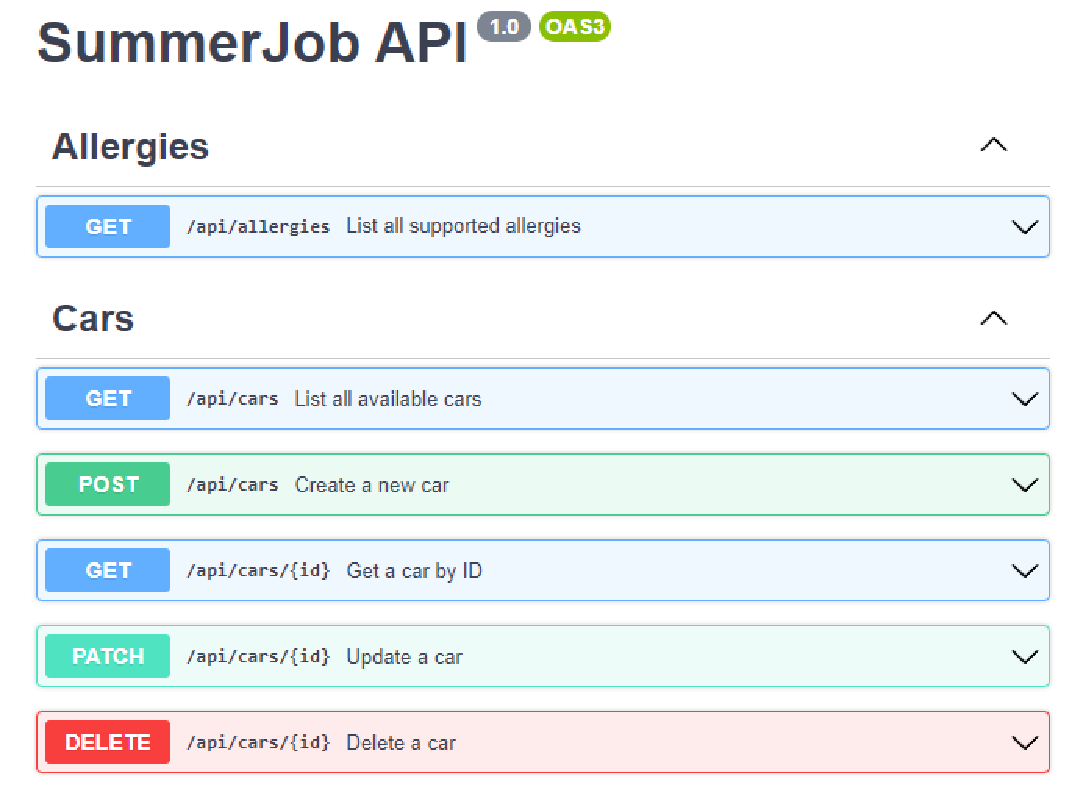
\includegraphics[width=1\textwidth]{chapters/images/swagger.pdf}
    \caption{Swagger dokumentace API}
    \label{fig:swagger}
\end{figure}

\subsection{Přihlášení}

Ověření uživatele není možné plně implementovat pomocí REST API, protože je nutné odeslat e-mail s přihlašovacím odkazem.
Je však možné přes API vyžádat odeslání e-mailu s přihlašovacím odkazem. Tento způsob využívá i webová aplikace, která při pokusu o přihlášení
vyžádá odeslání e-mailu a zobrazí uživateli další instrukce. Tento API endpoint spravuje knihovna NextAuth.js. Pro zvýšení bezpečnosti využívá knihovna
jednorázové CSRF tokeny. 

\subsection{Optimalizace}

Pro snížení objemu přenesených dat a zvýšení rychlosti odezvy API byly využity HTTP hlavičky \texttt{ETag}, \texttt{Last-Modified} a \texttt{If-None-Match}, které umožňují
posílat data pouze v případě, že jsou novější, než které má klient lokálně k dispozici.
Každý požadavek na API vrací v hlavičce ETag hash dat, která byla vrácena. Při dalším požadavku je možné v hlavičce If-None-Match poslat tento hash,
čímž se server rozhodne, zda vrátí data nebo pouze hlavičku s HTTP kódem 304 Not Modified. Tento způsob je využíván pro všechny požadavky, které vrací data.
Přenesená data jsou také komprimována pomocí gzip.

V případě opakovaných požadavků na stránce s plánem, které probíhají automaticky každou sekundu, se jedná o přenos přibližně 40 kB dat oproti
přibližně 5 MB za minutu, které by byly přeneseny bez využití těchto hlaviček. To umožňuje udržovat zobrazený plán stále aktuální i při pomalém či objemově limitovaném
připojení k internetu.
